
\documentclass[10pt,a4paper]{article}

\usepackage[a4paper,margin=0.7cm]{geometry}
\usepackage{graphicx}
\usepackage{xcolor}
\usepackage[hidelinks]{hyperref}
\usepackage{enumitem}

\pagenumbering{gobble}
\setlength{\parindent}{0pt}
\setlength{\fboxsep}{0pt}
\setlist[itemize]{leftmargin=1.2em,itemsep=2pt,topsep=2pt}

\definecolor {sidebar}{HTML}{DDD4C4}
\definecolor{accent}{HTML}{7A563D}
\definecolor{soft}{HTML}{F8F5F0}

\begin{document}

\noindent
\colorbox{sidebar}{
\begin {minipage}[t][27.5cm][t]{0.30\textwidth}
\vspace{0.6cm}

\begin{center}
    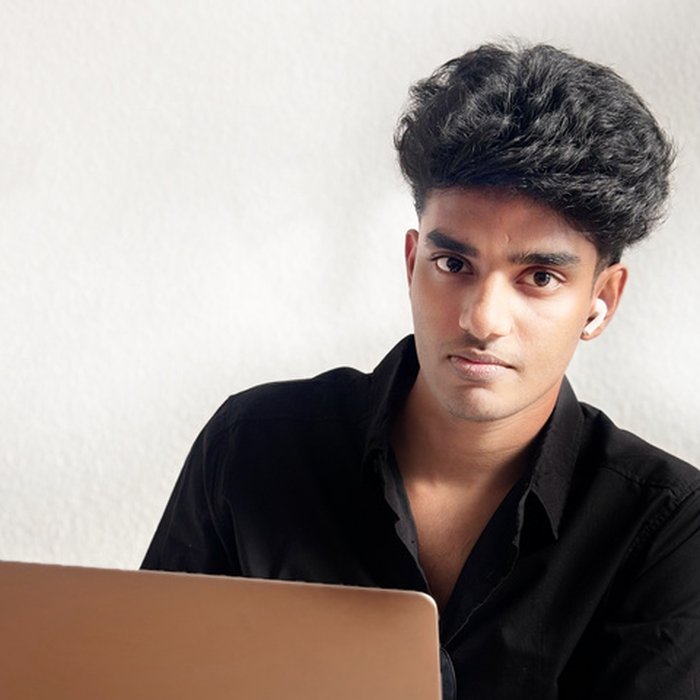
\includegraphics[width=3.4cm]{profile.png}
\end{center}

\vspace{0.4cm}

\hspace{0.35cm}
\begin{minipage}{0.78\textwidth}

{\large \textbf{Contact}}

\vspace{0.2cm}

Phone: +49 176 24734571\\
Email: \href{mailto:arjunbijoy1917r@gmail.com}{arjunbijoy1917r@gmail.com}\\
LinkedIn: \href{https://linkedin.com/in/arjun-bijoy-0b93b8380}{linkedin.com/in/arjun-bijoy-0b93b8380}\\
GitHub: \href{https://github.com/arjunbijoy1917r-cmyk}{github.com/arjunbijoy1917r-cmyk}\\
Portfolio: \href{https://github.com/arjunbijoy1917r-cmyk/computer-science-lab.git}{computer-science-lab}\\
Location: Berlin, Germany

\vspace{0.5cm}

{\large \textbf{Education}}

\vspace{0.2cm}

\textbf{Bachelor of Software Engineering}\\
GISMA University of Applied Sciences\\
Berlin, Germany\\
Current student

\vspace{0.25cm}

\textbf{Higher Secondary Education}\\
Bio-Maths, India\\
Completed in 2024

\vspace{0.5cm}

{\large \textbf{Skills}}

\vspace{0.2cm}

\begin{itemize}
    \item Python basics
    \item Java basics
    \item HTML and CSS
    \item SQL databases
    \item Basic LaTeX
    \item Problem solving
    \item Teamwork
\end{itemize}

\vspace{0.4cm}

{\large \textbf{Languages}}

\vspace{0.2cm}

\textbf{Malayalam} - Mother tongue\\
\textbf{English} - Good communication\\
\textbf{German} - Basic to intermediate, still improving

\end{minipage}
\end{minipage}
}
\hfill
\begin{minipage}[t][27.5cm][t]{0.66\textwidth}

\vspace{1.4cm}

\colorbox{soft}{
\begin{minipage}{0.96\textwidth}
\vspace{0.7cm}
{\Huge \textbf{ARJUN BIJOY}}\\
{\Large \textcolor{accent}{Software Engineering Student}}
\vspace{0.7cm}
\end {minipage}
}

\vspace{0.6cm}

I am a Software Engineering student studying at GISMA University of Applied Sciences in Berlin. I am developing my skills in programming, web development, and databases.

\vspace {0.3cm}

{\Large \textbf{Profile}}\\[-0.1cm]
\textcolor{accent}{\rule{1.5cm}{1pt}}

\vspace{0.2cm}

I am interested in technology, software development, and solving practical problems. I have worked on academic projects using Python and SQL. These projects helped me understand programming logic, database design, project structure, and how to organise technical work. I am still developing my skills.

\vspace{0.3cm}

{\Large \textbf{Projects}}\\[-0.1cm]
\textcolor{accent}{\rule{1.5cm}{1pt}}

\vspace{0.2cm}

\textbf{Python University System}\\
Python project based on a university system for organising data entry.\\
\href{https://github.com/arjunbijoy1917r-cmyk/python-university-system}{github.com/arjunbijoy1917r-cmyk/python-university-system}

\vspace{0.25cm}

\textbf {University Database Project}\\
SQL database project based on a university management system. It includes tables, sample data, relationships, and basic queries.\\
\href{https://github.com/arjunbijoy1917r-cmyk/university_database_project}{github.com/arjunbijoy1917r-cmyk/university\_database\_project}

\vspace{0.3cm}

{\Large \textbf{Academic and Technical Exercises}}\\[-0.1cm]
\textcolor{accent}{\rule{1.5cm}{1pt}}

\vspace{0.2cm}

\begin {itemize}
    \item Practiced beginner-level exercises in Python, HTML, CSS, SQL, and LaTeX.
    \item Created simple web pages and database-related project files.
    \item Learned how to organise project folders and upload work to GitHub.
\end{itemize}

\vspace{0.3cm}

{\Large \textbf{Portfolio}}\\[-0.1cm]
\textcolor{accent}{\rule{1.5cm}{1pt}}

\vspace{0.2cm}

\textbf{Computer Science Lab Portfolio}\\
This portfolio contains my computer science lab work and learning progress.\\
\href{https://github.com/arjunbijoy1917r-cmyk/computer-science-lab.git}{github.com/arjunbijoy1917r-cmyk/computer-science-lab.git}

\vspace{0.3cm}

{\Large \textbf{Additional Information}}\\[-0.1cm]
\textcolor{accent}{\rule{1.5cm}{1pt}}

\vspace{0.2cm}

\textbf{Nationality:} Indian\\
\textbf{Date of Birth:} 02 August 2006

\end{minipage}


\end{document}

